\documentclass[12pt, titlepage]{article}

\usepackage{array}
\newcolumntype{L}[1]{>{\raggedright\let\newline\\\arraybackslash\hspace{0pt}}m{#1}}
\usepackage{bookmark}
\usepackage{booktabs}
\usepackage{tabularx}
\usepackage{hyperref}
\usepackage{enumitem}
\usepackage{graphicx}
\usepackage{url}
\usepackage{fancyhdr}
\usepackage{graphicx}
\hypersetup{
    colorlinks,
    citecolor=black,
    filecolor=black,
    linkcolor=red,
    urlcolor=blue
}
\usepackage[round]{natbib}
\usepackage{titlesec}

\setcounter{secnumdepth}{4}

\titleformat{\paragraph}
{\normalfont\normalsize\bfseries}{\theparagraph}{1em}{}
\titlespacing*{\paragraph}
{0pt}{3.25ex plus 1ex minus .2ex}{1.5ex plus .2ex}

\title{SE 3XA3: Software Requirements Specification\\JSTanks}

\author{Team 6, JSTanks
		\\ Jiahao Li (li577)
		\\ Pavithran Pathmarajah (pathmap)
		\\ Viren Patel (patelvh3)
}

\date{\today}

\begin{document}

\maketitle
\pagenumbering{roman}
\tableofcontents
\listoftables
\listoffigures

\begin{table}[bp]
\caption{\bf Revision History}
\begin{tabularx}{\textwidth}{p{3cm}p{2cm}X}
\toprule {\bf Date} & {\bf Version} & {\bf Notes}\\
\midrule
September 29 & 0 & Initial Draft\\
September 29 & 0 & Initial Draft\\
September 29 & 0 & Initial Draft\\
December 02 & 1 & Reorganization and Amendment\\
\bottomrule
\end{tabularx}
\end{table}

\newpage

\pagenumbering{arabic}

\section{Project Drivers}
\subsection{The Purpose of the Project}
\subsubsection{The User Business or Background of the Project Effort}
The objective of this project is to expand the accessibility options for the famous
Tanks game. The game we will be working on is currently a stand-alone program
which requiring a Java interface to compile or any other means of manual
compilation. This can be an issue for a lot of users as they might not have the
necessary knowledge or have compatibility problems with their platform. Our plan
to transform this Java Program to a web-based application will rid of any issues
and allow users to experience playing the game without any difficulties. What
motivates us to go on with this project is the will to be a part of the game
development community which is a power station providing a great number of
options for people seeking entertainment through video games. This game is not a
serious problem and is not necessarily a significant business opportunity for
our host. This is because there are various versions of the Tanks game already
available online for users at the present moment. This however is only theory
based because the host popularity and traffic has a great impact on how
significant this game is in terms of business.
\subsubsection{Goals of the Project}
The ultimate service goal we are trying to achieve is to make easy access of the 
Tanks game for the users. We will be using JavaScript as our programming language 
in order to make the game runnable on a website. We will then decide on a host that 
will best suite our product and help popularize it.
\subsection{The Stakeholders}
\subsubsection{The Client}
The client for our product is the titleholder of the website which will be hosting our 
completed version of the Tanks game. Their role will be to review the final version 
of our product and share an interest in gaming entertainment.
\subsubsection{The Customers}
Our customer will be the general public seeking gaming
entertainment. The typical customer would have access to the Internet and a
computer platform (laptops or desktops). Although our product is suitable for
all age groups, children and teenagers are expected to make up the majority of
our customers.
\subsubsection{Other Stakeholders}
Developers:
\begin{itemize} 
\item 
JSTanks is the team of developers for this project. All developers will play a role in
redeveloping the Tanks game; transforming it from a Java application to a
website friendly game easily available to all potential customers.
\end{itemize} 
Professor and TAs of SE3XA3:
\begin{itemize} 
\item 
The professor and TAs of SE3XA3 help to develop the project and give comments
which improve the development of the project.
\end{itemize} 
Other Software Developers 
\begin{itemize} 
\item 
These are members of the general public, but what separates them from the rest 
is their interest in game/software development. This includes people who may be 
in our shoes; looking to redevelop an open source software or they could be complete 
beginners wanting to get into developing software using our product as a learning 
example.
\end{itemize}
\subsubsection{Hands-On Users of the product:}
Teenagers and University / College Students
\begin{itemize}
\item Use games as a means of entertainment
\item Novice in game development
\item Masters of gaming media and its consumption
\item Access to the product, majority age group 11 - 24
\end{itemize}
\subsubsection{Personas:}
\begin{description}[align=right,labelwidth=4cm]
\item [Name:] Luke Cage
\item [Age:]20
\item[Job:]Student
\item[Family:]Oliver Cage - Father, Felicity Cage - Mother
\item[Hobbies:]Educational Politics
\item[Residence:] North Bay, ON, Canada
\item[Favourite Food:] Poutine
\item[Favourite Music:] EDM   Alan walker
\item[Likes:]Tanks, Action, Flash Games
\item[Dislikes:] High tuition costs of post-secondary education 
\item[Preferred Holiday:] Niagara Falls, Canada
\item[Attitude to Technology:] Positive
\item[Attitude to Money:] Extremely Positive
\end{description}
\subsubsection{Priorities Assigned to Users}
\begin{itemize}
\item Key Users: Client, Customers
\item Secondary Users: other developers, general public
\item Unimportant Users: general public
\end{itemize}
\subsubsection{User Participation}
No participation is required from any users
\subsubsection{Maintenance Users and Service Technicians}
JSTanks\\
The Developers Team will be responsible for maintaining and changing the source
code for this product. They will also communicate with the client in order to
ensure the website has considerate uptime.
\subsection{Mandated Constraints}
\subsubsection{Solution Constraints}
 Description: The game shall be compatible
and be able to run on Mozilla Firefox 49.0.1 and -Google Chrome 53.0.2785.143
browsers.\\\\ Rationale: The game will not be updated for any previous versions
that might cause issues with the execution of the game client.\\\\ Fit
Criterion: The game shall be available to users with the mentioned browser
versions or any other versions which are compatible to run the game.\\\\
Description: The game shall only use HTML, CSS, and JavaScript for
implementation and execution.\\\\ Rationale: The client will not use any other
web related software and will have the correct versions of HTML, CSS, and
JavaScript. \\\\ Fir Criterion: The users shall be able to run the game with no
issues given they have the right version of JavaScript on their platform. \\\\
\subsubsection{Implementation Environment of the Current System}
\begin{figure}[hb]
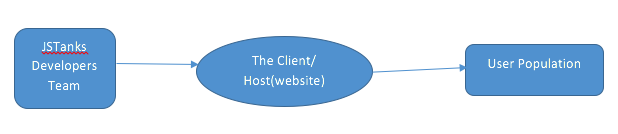
\includegraphics[width=\textwidth]{Fig1.png}
\caption{Implementation Environment  Diagram of the Current System} \label{fig:Fig1.png}
\end{figure}
\subsubsection{Partner and Collaborative Applications:} 
The product requires a
text editor for the HTML, CSS, and JavaScript implementation to take place in.
Because it is a web based software, it requires a browser with JavaScript and a
server provided by the client. There are no other partner and collaborative
applications for this product.
\subsubsection {Off-The-Shelf-Software:}
\begin{itemize}
\item Text editor i.e. Notepad++
\item A web browser i.e. Mozilla Firefox, Google Chrome
\item JavaScript for implementation
\end{itemize}
\subsubsection{Anticipated Workspace Environment:} 
There is no specific working
environments for this product, it can be used as long as there is a computer
desktop or a laptop (portability) and an internet connection.
\subsubsection{Schedule Constraints} 
The given deadline for the finished
product is December 8th, 2016. In addition, a proof of concept demonstration
requires a minimum amount of implementation done to be presented on the week of
October 17, 2016.
\subsubsection{Budget Constraints} 
There are no budget constraints to the
development of this product. However, a goal imposed upon ourselves as a team is
to use absolutely no money in the making of this product.
\subsubsection{Enterprise Constraints} 
There are no enterprises involved in the
product development. This game is free of charge and requires nothing more than
a computer platform and an internet connection.
\subsection{Naming Conventions and Terminology}
The terminology used in this project is given in table 2.  All abbreviations included in
the projection is on the left hand side of the table, and their meanings are on the right
hand side.
\begin{table}[h]
\caption{List of terminology} \label{tab:terminology}
\begin{tabular}{ | l | l |}
\hline
Acronym/Abbreviation  & Meaning\\\hline
JSTanks & Team Name\\\hline
JSTanks & Project Name\\\hline
JS & JavaScript\\\hline
HTML & Hypertext mark up language\\\hline
CSS & Cascading style sheets\\\hline
git & Git Lab\\\hline
API & Application program interface\\\hline
GUI & Graphical user interface\\\hline
AI & Artificial intelligence\\\hline
PC & Personal computer\\\hline
\end{tabular}
\end{table}
\subsection{Relevant Facts and Assumptions}
The project is base on an existing
application called tanks which is an open source with 684 lines of code. The aim
is to convert such game from the local PC version to the website version using
JS which allow users to enjoy the game without downloading.\\\\ The game is
intend to be run on the web page, so we assume that modern computers which are
capable of running latest browsers is available to users. Since the game take
the keyboard as the input tool, a keyboard is also required to play the game.
\section{Functional Requirements}
\subsection{The Scope of the Work and the Product}
\subsubsection{The Context of the Work}
\begin{figure}[hp]
\includegraphics[width=\textwidth]{Fig2.png}
\caption{The Context of the Work} \label{fig:Fig2.png}
\end{figure}
The major part of our project is a web-base Tanks game. We will port the original
game with JavaScript to make it work on broswers. The game will take the keyboard
input as the input and display in the broswer provide users a visual game play.
\subsubsection{Work Partitioning}
BUC Cases do not apply
\subsubsection{Individual Product Use Cases}
\begin{enumerate}
\item When the user clicks `start a new game' in the menu, the whole web page gets
 refreshed which makes all stuff in the game back to their initial positions.
\item When the user clicks `pause' in the menu, the game come into a pause state.
 All stuff in the game freeze and stay in their temporal position until the 
 button `continue' in the menu is clicked.
\item When the user clicks `continue' in the menu, the game is activated from 
the pause state that all stuff run as the routine if it was the pause state 
before the click. And the click of  `continue' cause no effect if it was not the 
pause state before the click.
\item When the user click the different `level' in the menu, the speed of tanks 
controlled by the AI changes in the game. The higher the level is, the higher 
the speed is.
\item When the user clicks `introduction' in the menu, the web page pops up a 
window with the information of the game in it.
\item When the user clicks `quit' in the menu, the game comes to the end state 
that the GUI turns into black with only the menu on it.
\item When the user presses the `up', `down', `left' or `right' key on the 
keyboard, the tank controlled by the user moves to the exact direction according 
to the key. If the user keep pressing the key, the tank keeps moving until it 
hits the wall or the boundary of the map.
\item When the user press the `F' key on the keyboard, the tank controlled by the
 user launches a bullet. The bullet keeps moving and disappears when it hits 
 another tank, a wall or the boundary of the map.
\item When the bullet launched by the user's tank hits another tank controlled 
by the AI, that tank and the bullet disappear all together at the same time.
\item When the bullet hits a brick wall, the wall and the bullet disappear all 
together at the same time.
\item When the bullet hits a steel wall, the bullet disappears and the steel 
wall keep existing in the same position.
\item When the tank controlled by the user or the home base is hit by the 
bullet which is launched by the tank controlled by the AI, one tenth of blood 
in the blood bar decreases.
\item When the blood bar is empty which means that the home base is destroyed, 
the web page pops up a window showing that the game is over.
\item When the tank controlled by the user cross over a heart, one-tenth of 
blood increases in the blood bar. The blood does not increase if the blood bar 
is full.
\item When the tank controlled by the user is the only tank in the map, the web 
page pops up a window showing that the user wins the game, and then the game 
come to the end state.
\end{enumerate}
\subsection{Functional Requirements}
\subsubsection{Functional Requirements 1} The executable HTML file shall create a new browser window.\\Priority: High
\subsubsection{Functional Requirements 2} The HTML shall be executed by a browser with JavaScript functionality.\\Priority: High
\subsubsection{Functional Requirements 3} The game shall have a standby state in which it waits for user input.\\Priority: Medium
\subsubsection{Functional Requirements 4} The menu with four sections which are `game', `pause/continue', `level' and
 `introduction' shall shows up in the standby state.\\Priority: Low
\subsubsection{Functional Requirements 5} The sub menu of `game' section which has choices of `start a new game' and 
`quit' shall shows up when the `game' section is clicked.\\Priority: Medium
\subsubsection{Functional Requirements 6} The sub menu of  `pause/continue' section which has choices of `pause‘ and  
`continue' shall shows up when the `pause/continue' section is clicked.\\Priority: Medium
\subsubsection{Functional Requirements 7} The sub menu of  `level' section which has choices of `level 1', `level 2',
 and `level 3' shall shows up when the `level' section is clicked.\\Priority: Low
\subsubsection{Functional Requirements 8} The game shall be reset and start when `start a new game' is clicked.\\Priority: Medium
\subsubsection{Functional Requirements 9} The game shall close the window when `quit' is clicked.\\Priority: Medium
\subsubsection{Functional Requirements 10} the game shall come to the pause state when `pause' is clicked.. All stuff 
in the game shall freeze and stay in the temporal positions in the pause state.\\Priority: Medium
\subsubsection{Functional Requirements 11} All stuff frozen by the `pause' button in the game shall be activated and
 back into the routine when `continue' is clicked.\\Priority: Medium
\subsubsection{Functional Requirements 12} The click of the `continue' button shall have no effect if the game is not
 in the pause state.\\Priority: Medium
\subsubsection{Functional Requirements 13} The AI shall control tanks to move and fire randomly when the game starts.\\Priority: High
\subsubsection{Functional Requirements 14} The moving speed of tanks controlled by the AI shall change when `level 1'
, `level 2' or `level 3' is clicked. The higher the level is, the higher the speed
 it.\\Priority: Medium
\subsubsection{Functional Requirements 15} The `level 1' shall be chosen as the default speed of tanks when the game 
starts.\\Priority: Low
\subsubsection{Functional Requirements 16} The window with the information of the game in it shall pops up when 
`introduction' is clicked.\\Priority: Low
\subsubsection{Functional Requirements 17} The tank controlled by the user shall move left, right, up or down when 
the left, right, up or down key on the keyboard is pressed. The tank shall keep
 moving when the key is kept pressing until the tank hits the wall or the 
 boundary of the map.\\Priority: High
\subsubsection{Functional Requirements 18} A bullet shall be launched and move along the direction that the tank
 faces to when the `F' on the keyboard is pressed. One bullet shall be launched 
 every time that user press `F'.\\Priority: High
\subsubsection{Functional Requirements 19} When the bullet launched by the user's tank hit another tank, that tank 
shall disappear with the bullet at the same time.\\Priority: Medium
\subsubsection{Functional Requirements 20} When the bullet launched by the user's tank hit a brick wall, the brick 
wall shall disappear with the bullet at the same time.\\Priority: Medium
\subsubsection{Functional Requirements 21} When the bullet launched by the user's tank hit a steel, the bullet shall 
disappear and the steel wall shall disappear after being hit for three times.\\Priority: Medium
\subsubsection{Functional Requirements 22}There shall be a blood bar for the home base under the map. When 
the bullet launched by the tank of the AI hits the  home base, one-eighth of the blood in the blood bar of the home base 
shall decrease.\\Priority: Medium
\subsubsection{Functional Requirements 23} There shall be a blood bar for the user's tank under the map.When 
the bullet launched by the tank of the AI hits the user's tank, one-sixth of blood in the blood bar of the user's tank shall 
decrease.\\Priority: Medium
\subsubsection{Functional Requirements 24} A window shall pops up to show that the game is over and the game shall
 comes to the end state if the user's tank or the home base is destroyed.\\Priority: High
\subsubsection{Functional Requirements 25} The window shall pops up to show that the user wins the game and the game
 comes to the end state if the user's tank is the only one left in the map.\\Priority: High
 \subsubsection{Functional Requirements 26} There shall not be a score for the user's tank, because the only way that
 the user win the game is to protect the home base and itself and destroy all tanks of the AI. \\Priority: High
\section{Non-functional Requirements}
\subsection{Look and Feel Requirements}
\subsubsection{Appearance Requirements}
The game shall acknowledge the client hosting it on a website by showing its
credentials upon starting up. The game should be visually attractive and have
appealing colour schemes. The game will have many tanks other than the user
tank. The player tank will be coloured differently and all AI tanks will be
coloured the same to make it easier for the player to tell the difference. There
shall be brick sprites which make up the player?s home base and graphics for
bullets fired from all tanks.\\Priority: Medium
\subsubsection{Style Requirements}
JS Tanks shall colour the tanks and the background so that they do not make it
hard for the user to focus on the screen. The game shall have a menu with
different options that the player can go through. i.e. Play, Instructions, Quit.\\Priority: High
\subsection{Usability and Humanity Requirements}
\subsubsection{Ease of use requirements}
JS Tanks being a very simplistic game shall be very ease to play for all users. 
The interface as well as the controls shall be very basic, but at the same time, 
the gameplay should be satisfying for the player. \\Priority: High
\subsubsection{Personalization and Internationalization Requirements}
This is not applicable to this game. \\Priority: Low
\subsubsection{Learning Requirements}
The user requires no further knowledge than to be able to open the browser.\\Priority: High
\subsubsection{Understandability and Politeness Requirements}
The user should know simple English to surf through the menu and read 
instructions.\\Priority: High
\subsubsection{Accessibility Requirements}
The user should be able to access the game from any platform with a web browser 
supporting JavaScript.\\Priority: High
\subsection{Performance Requirements}
JS Tanks should be able to operate with minimal hardware specific requirements 
for the basis of the project is stray away from specific and high end hardware. 
The game should be able to operate with little input latency and no notable 
frame rates.\\Priority: Medium
\subsection{Operational and Environmental Requirements}
The game should run on Chromium web-browsers and Firefox browsers, across 
operating systems most notably Windows and OSX systems. The game should run 
within the web browser and require no connection to a server for processing.\\Priority: High
\subsection{Maintainability and Support Requirements}
The code for the game should be simple and easy to understand and breakdown 
to help those maintaining the code or others whom plan to learn from it or 
build their own Java Script application.\\Priority: Medium
\subsection{Security Requirements}
The game should not access nor compromise user data, nor should it access or 
compromise the hosting entities data.\\Priority: High
\subsection{Cultural Requirements}
JS Tanks shall be available only in English and contain no directly offensive 
remarks to any culture or nation.\\Priority: High
\subsection{Legal Requirements}
The game must abide by Canada's Anti-Spam Legislation.\\Priority: High
\\\\The game should try to meet the standards set by Canada's Accessibility 
Legislation.\\Priority: High
\subsection{Health and Safety Requirements}
The game should not cause any health and safety problem for users both physically and mentally.
\\Priority: High
\section{Project Issues}
\subsection{Open Issues}
Currently there are two issues plaguing our development of this project. Firstly
the members of JSTanks are not particularly affluent in Java Script which is
slowing down development as the team must learn as it develops. Secondly,
deriving from the first issue the team is unsure of Java Script in its ability
to create and handle objects, this issue will be looked into quickly; if Java
Script is unable to create or handle objects then a more procedural approach
will need to be followed.
\subsection{Off-the-Shelf Solutions}
\subsubsection{Ready Made}
Ready made solutions which can be used are simple parsers to convert to Java
Script but to do this, the java must first be parsed into another language for
no direct Java to Java Script parser is available and by doing multiple language
conversion efficiency can easily be lost.
\subsubsection{Reusable Components}
The components of the original project cannot be re-used due to the language and
platform barrier, but the existing algorithms can be broken down and re-used but
this is to be determined.
\subsubsection{Products that can be copied}
Currently there is no full product which may be duplicated but what can be
copied are Java Script tutorials for specific functions which can be merged
together to create an acceptable result.
\subsection{New Problems}
\subsection{Tasks}
\begin{itemize}
\item Break down original project into workable components
\item Convert Java components into algorithms and then into Java Script
\item Merge components together to make fluent and efficient game
\end{itemize}
\subsection{Migration to the New Product}
There is no product being replaced, and thus no migration is required.
\subsection{Risks}
The only potential risk the development process might have is that we are
learning new languages; HTML, CSS, and JavaScript. This learning period will
take some space in our Development timeline and might under specific
circumstances cause delays to the project schedule. This in turn, could
compromise the quality of the final product. i.e. poor gameplay.
\subsection{Costs}
Not applicable as there are no set constraints for cost.
\subsection{User Documentation and Training}
\subsubsection{User Documentation Requirements}
Not Applicable.
\subsubsection{Training Requirements}
The game menu shall have an option giving a brief explanation of game and 
controls. 
\subsection{Waiting Room}
\begin{itemize}
\item In-Game Audio
\item Mobile edition
\item Multiplayer
\end{itemize}
\subsection{Ideas for Solutions}
Ideas of solutions will be figured out after learning more knowledge beyond the course.
\bibliographystyle{plainnat}
\newpage
\section{Appendix}
\subsection{Business Data Model and Data Dictionary}
\subsubsection{Business data Model}
\begin{figure}[hp]
\includegraphics[width=\textwidth]{Fig3.png}
\caption{Business data Model} \label{fig:Fig3.png}
\end{figure}
\subsubsection{Data Dictionary}
\paragraph{Artificial Intelligence}
Attributes: Difficulty of AI
\\\\Relationships:  Connected to the Tank class such that once it is initiated 
as a tank, location, health and direction can be tracked
\\\\Inputs: Tank locations, Player location, Base Location
\\\\Outputs: Tank directional movement, Tank Attacks
\paragraph{Keyboard Input}
Attributes: Current and last, inputs
\\\\Relationships: Connected to the Tank class such that once a player makes a 
move it can be passed onto there respective tank
\\\\Inputs: Keyboard input
\\\\Outputs: Tank directional movement, Tank attacks
\paragraph{Tank}
Attributes: Location, movement, attack
\\\\Relationships: Connected to the Tiles class to track if it can move or if 
there is a wall, base or tank in its way
\\\\Inputs: Directional Movement, Tiles beside the tank tile
\\\\Outputs: Moved to location
\paragraph{Walls}
Attributes: Location
\\\\Relationships: Connected to the Tiles class such that its health can be 
tracked and such that tanks can recognize there is a wall
\\\\Inputs: None
\\\\Outputs: None
\paragraph{Base}
Attributes: Location
\\\\Relationships: Connected to the Tiles class such that its health can be 
tracked and such that tanks can recognize where the base is
\\\\Inputs: Destroyed
\\\\Outputs: End-Game
\paragraph{Tiles}
Attributes: Health, track adjacent tiles
\\\\Relationships: Connected to all three tile types and acts as a game board
\\\\Inputs: moved locations, projectile attack on a tile
\\\\Outputs: Health, destroyed tile, adjacent tiles, launch attack
\paragraph{Projectiles}
Attributes: Direction, strength
\\\\Relationships: Connected to tiles, such that tile health can be updated
\\\\Inputs: Attack launched in direction
\\\\Outputs: Tile hit by attack
\paragraph{End Game}
Attributes: None
\\\\Relationships: Attached to Base which when destroyed ends the game
\\\\Inputs: Game Over
\\\\Outputs: Score and menu

\end{document}